\documentclass[12pt,letterpaper,oneside,openright]{book}


%%%%%%%%%%%%%%%%%%%%%%%%%%%%%%%%%%%%%%%%%%%%%%
%% Page Layouts: Margins and Page Numbering %%
%%%%%%%%%%%%%%%%%%%%%%%%%%%%%%%%%%%%%%%%%%%%%%

\pagestyle{plain}  % Centering the page number at the bottom of the page
\usepackage[left=1.5in,right=1.0in,top=1.0in,bottom=1.0in,includefoot,heightrounded]{geometry}  % Margins by the UH NSM thesis formatting
\usepackage[doublespacing]{setspace}
\usepackage[hidelinks]{hyperref}
\usepackage{multicol}
\usepackage{tocbibind}
\usepackage{tikz} % for drawing Feynman diagrams
\usepackage{amsmath} % for mathematics expressions


%%%%%%%%%%%%%%%%%%%%%%%%%%%%%%%%%%%%%%%%
%% Font Selection: Palatino or Minion %%
%%%%%%%%%%%%%%%%%%%%%%%%%%%%%%%%%%%%%%%%

%\usepackage{palatino}
\usepackage{libertine}

%\usepackage{fontspec} % For loading fonts
%\setmainfont{Minion Pro} % Main document font

\newcommand{\HRule}{\rule{\linewidth}{0.5mm}}


%\title{Neutron Production by Cosmic Muons at Daya Bay}


\begin{document}

% Define styles for the different kind of edges in a Feynman diagram
\tikzset{
    photon/.style={decorate, decoration={snake}, draw=red},
    electron/.style={draw=blue, postaction={decorate},
        decoration={markings,mark=at position .55 with {\arrow[draw=blue]{>}}}},
    gluon/.style={decorate, draw=magenta,
        decoration={coil,amplitude=4pt, segment length=5pt}} 
}

\frontmatter
	\pagenumbering{roman}
	\begin{titlepage}
\begin{center}

% Upper part of the page. The '~' is needed because \\
% only works if a paragraph has started.
%\includegraphics[width=0.15\textwidth]{./logo}~\\[1cm]

%\textsc{\LARGE Neutron Production By Cosmic Muons}\\[1.5cm]

%\textsc{\Large Final year project}\\[0.5cm]
\begin{description}
\bigskip
\bigskip
\bigskip
\bigskip
\bigskip
\end{description}

% Title
{ \huge \bfseries Neutron Production By Cosmic Muons \\[0.4cm] }

\HRule \\[1.0cm]

A Dissertation Presented to\\
the Faculty of the Department of Physics\\
University of Houston\\[1.0cm]

\HRule \\[1.0cm]

In Partial Fulfillment\\
of the Requirements for the Degree\\
Doctor of Philosophy\\[1.0cm]

\HRule \\[1.0cm]

By\\
Shih-Kai Lin\\
August 2014

% Author and supervisor
%\begin{minipage}{0.4\textwidth}
%\begin{flushleft} \large
%\emph{Author:}\\
%John \textsc{Smith}
%\end{flushleft}
%\end{minipage}
%\begin{minipage}{0.4\textwidth}
%\begin{flushright} \large
%\emph{Supervisor:} \\
%Dr.~Mark \textsc{Brown}
%\end{flushright}
%\end{minipage}

%\vfill

% Bottom of the page
%{\large \today}

\end{center}
\end{titlepage}
	\setcounter{page}{2}
	
\begin{center}

% Upper part of the page. The '~' is needed because \\
% only works if a paragraph has started.
%\includegraphics[width=0.15\textwidth]{./logo}~\\[1cm]

%\textsc{\LARGE Neutron Production By Cosmic Muons}\\[1.5cm]

%\textsc{\Large Final year project}\\[0.5cm]
\begin{description}
\bigskip
\end{description}

% Title
{ \huge \bfseries Neutron Production By Cosmic Muons \\[0.4cm] }

\end{center}


\begin{flushright}
  \begin{minipage}[c]{0.6\textwidth}
  \vspace{2.0cm}
  
  \begin{spacing}{0}
  \rule{\textwidth}{0.5mm}
  \textbf{Shih-Kai Lin}\\
  \end{spacing}
  
  \vspace{1.5cm}
  APPROVED:\\
  \vspace{\baselineskip}
  
  \begin{spacing}{0}
  \rule{\textwidth}{0.5mm}
  \textbf{Dr. Kwong Lau}\\
  \end{spacing}
  \vspace{2.4cm}
  
  \begin{spacing}{0}
  \rule{\textwidth}{0.5mm}
  \textbf{Dr. Ed Hungerford}\\
  \end{spacing}
  \vspace{2.4cm}
  
  \begin{spacing}{0}
  \rule{\textwidth}{0.5mm}
  \textbf{Dr. Donald Kouri}\\
  \end{spacing}
  \vspace{2.4cm}
  
  \begin{spacing}{0}
  \rule{\textwidth}{0.5mm}
  \textbf{Dr. Lawrence S. Pinsky}\\
  \end{spacing}
  \vspace{2.4cm}
  
  \begin{spacing}{0}
  \rule{\textwidth}{0.5mm}
  \textbf{Dr. Rene Bellwied}\\
  \end{spacing}
  \vspace{2.4cm}
  
  \begin{spacing}{0}
  \rule{\textwidth}{0.5mm}
  \textbf{Dr. Rene Bellwied}\\
  \end{spacing}
  \vspace{2.4cm}
  
  \begin{spacing}{0}
  \rule{\textwidth}{0.5mm}
  \textbf{Dean, College of Natural Sciences and Mathematics}\\
  \end{spacing}
  
  \end{minipage}
\end{flushright}
	\input{mainmatter/abstract_title.tex}
	\chapter*{\centering Abstract}
My abstract goes here.
\addcontentsline{toc}{chapter}{Abstract}
	\tableofcontents
	\listoffigures
	\listoftables

\mainmatter
  \chapter{Introduction}

\section{Overview of Neutrino Physics}

On December 4 1930, in an open letter addressed to "Dear Radioactive Ladies and Gentlemen" attempting to salvage one of the most fundamental principles in physics, energy conservation, W. Pauli postulated a neutral weakly interacting particle which is later dubbed \emph{neutrino} and opened up neutrino physics. In 1934, E. Fermi formulated the first successful theory of weak interactions, the Fermi theory of $\beta$-decay.

\section{Neutrino Oscillation and \texorpdfstring{$\theta_{13}$}{theta13}}

\subsection{Neutrino Mixing and Neutrino Oscillation}
According to the Standard Model of Particle Physics, there are 3 flavors of neutrinos, namely, $\nu_e$, $\nu_\mu$ and $\nu_\tau$. These are the eigenstates when neutrinos take part in weak interactions. However, these are not the eigenstates when neutrinos propagate freely in space. Since neutrinos have minute but nonzero mass, there are 3 mass eigenstates and the relation between flavor and mass eigenstates can be written as
\begin{equation}
\left( \begin{array}{c} \nu_e \\ \nu_\mu \\ \nu_\tau \end{array} \right)
=
\begin{pmatrix}
U_{e1} & U_{e2} & U_{e3} \\
U_{\mu1} & U_{\mu2} & U_{\mu3} \\
U_{\tau1} & U_{\tau2} & U_{\tau3}
\end{pmatrix}
\left( \begin{array}{c} \nu_1 \\ \nu_2 \\ \nu_3 \end{array} \right)
\end{equation}

The unitary matrix $[U_{lj}]$ is called PMNS matrix named after physicists B. Pontecorvo, Z. Maki, M. Nakagawa, and S. Sakata and can be parametrized by

\allowdisplaybreaks
\begin{align}
U_{PMNS}=
\begin{pmatrix}
c_{12}c_{13} & s_{12}c_{13} & s_{13}e^{-i\delta} \\
-s_{12}c_{23}-c_{12}s_{23}s_{13}e^{-i\delta} & c_{12}c_{23}-s_{12}s_{23}s_{13}e^{-i\delta} & s_{23}c_{13} \\
s_{12}s_{23}-c_{12}c_{23}s_{13}e^{-i\delta} & -c_{12}s_{23}-s_{12}c_{23}s_{13}e^{-i\delta} & c_{23}c_{13}
\end{pmatrix}
\begin{pmatrix}
e^{i\phi_1} & 0 & 0 \\
0 & e^{i\phi_2} & 0 \\
0 & 0 & 1
\end{pmatrix}
\end{align}

If an electron antineutrino $\bar{\nu}_e$ is produced at the source and propagates in space, at a distance $L$ away from the source the survival probability, i.e. the probability that the neutrino doesn't change to other flavors, is
\allowdisplaybreaks
\begin{align}
P(\bar{\nu}_e\rightarrow\bar{\nu}_e)=1-c^4_{13}\sin^22\theta_{12}\sin^2\Delta_{21}-c^2_{12}\sin^22\theta_{13}\sin^2\Delta_{31}-s^2_{12}\sin^22\theta_{13}\sin^2\Delta_{32}
\end{align}

Among the three mixing angles $\theta_{13}$ was the only unknown parameter, and the goal of Daya Bay experiment was to measure $\sin^22\theta_{13}$ with $0.01$ sensitivity at $90\%$ confidence level.


\subsection{Neutrino Flux and Energy Spectrum}

Nuclear power is generated by fission reactions mainly from 4 kinds of isotopes, namely $^{235}$U, $^{239}$Pu, $^{238}$U and $^{241}$Pu. The fission products then undergo beta decay and generate neutrinos. Each fission reaction on average produces about 6 neutrinos. The detailed neutrino flux and energy spectrum at a particular time depend on the composition of the isotopes, the total reactor thermal power, the fission rate of individual isotopes and the spectrum of the individual isotopes. The number of neutrinos released by the reactor per unit time is
\begin{equation} \label{eq:neutrino_flux}
  \phi(E)=\frac{W_{th}}{\sum\limits_{i=1}^4f_ie_i}\sum\limits_{i=1}^4f_iS_i(E)
\end{equation}
where $i$ runs over the four main isotopes, $W_{th}$ is the total thermal power, $f_i$ is the fission fraction, $e_i$ is the fission energy release and $S_i(E)$ is the neutrino energy spectrum.

The fission fraction of each isotope and the total thermal power are monitored and the weekly averaged numbers are offered by the nuclear power plant. $e_i$ is the part of the fission energy that converts into heat. Typical values at the midpoint of the reactor operation period is given in Table~\ref{table:thermal_fission_energy}~\cite{Kopeikin2004}.
\begin{table}
	\centering
	\begin{tabular}{|c|c|}
	\hline
	isotope & $e_i$ (MeV/fission) \\
	\hline
	$^{235}$U & 201.92 ± 0.46 \\
	$^{238}$U & 205.52 ± 0.96 \\
	$^{239}$Pu & 209.99 ± 0.60 \\
	$^{241}$Pu & 213.60 ± 0.65 \\
	\hline
	\end{tabular}
	\caption{Typical thermal fission energy $e_i$ at the midpoint of the reactor operation period.}
	\label{table:thermal_fission_energy}
\end{table}

The antineutrino spectra $S_i(E)$ can be calculated theoretically. A three parameter calculation was done by Vogel and Engel~\cite{Vogel1989}. Figure~\ref{figure:isotope_antineutrino_spectra} shows the spectra of the four dominant isotopes. $^{238}$U produces the most antineutrinos per fission while $^{239}$Pu produces the least.
\begin{figure}
	\centering
	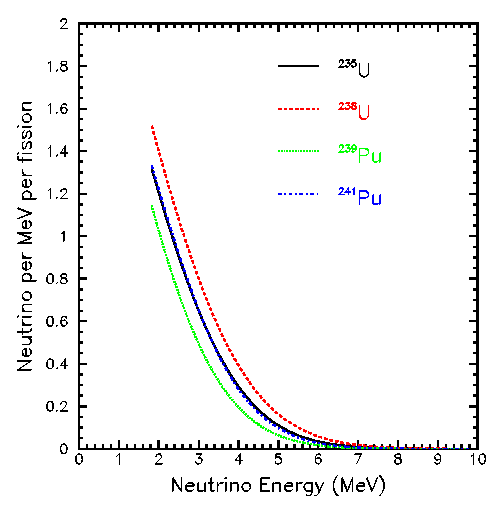
\includegraphics[width=.5\textwidth]{figures/chap1/isotope_antineutrino_spectra.eps}
	\caption{Calculated antineutrinos spectra for each dominant isotope.}
	\label{figure:isotope_antineutrino_spectra}
\end{figure}


\subsection{\texorpdfstring{$\bar{\nu}_e$}{Electron Antineutrino} Detection}
Daya Bay utilizes the renowned Cowan–Reines method of prompt-delayed coincidence to detect $\bar{\nu}_e$. The reaction involved in this method is the inverse beta decay (IBD),
\begin{equation}
	\bar{\nu}_e+p\longrightarrow e^++n
\end{equation}
The positron is quickly annihilated by an electron and releases photons which constitute the prompt signal. The neutron propagates in the target medium, slows down mainly by collisions with protons and finally gets captured by some nucleus which in turn de-excites and releases photons constituting the delayed signal. Such prompt-delayed coincidence forms a very definitive $\bar{\nu}_e$ signature and greatly suppresses backgrounds.

The antineutrino event rate is given by
\begin{equation}
	R=\int \epsilon(E)P_{\bar{\nu}_e\rightarrow\bar{\nu}_e}(L,E)\frac{N_p\sigma(E)}{4\pi L^2}\phi(E)dE
\end{equation}
where $\epsilon$ is the antineutrino detection efficiency, $P_{\bar{\nu}_e\rightarrow\bar{\nu}_e}$ is the antineutrino survival probability, $N_p$ is the number of protons in the detector, $\sigma$ is the IBD total cross section, $L$ is the distance from the reactor core to the detector and $\phi$ is the number of released antineutrinos per unit time given in Eq.~\ref{eq:neutrino_flux}.

$P_{\bar{\nu}_e\rightarrow\bar{\nu}_e}$ depends on $\sin^22\theta_{13}$ which we want to infer from the measured IBD rates. $\epsilon$, $N_p$ and $L$ are measured by auxiliary methods and instruments which will be detailed later. The total cross section of the IBD reaction in the limit of infinite nucleon mass can be written as~\cite{Vogel1999}
\begin{equation}
	\sigma^{(0)}_{tot}=0.0952\times 10^{-42} \left( \frac{E^{(0)}_ep^{(0)}_e}{1 MeV^2}\right) cm^2
\end{equation}
where $E^{(0)}_e$ and $p^{(0)}_e$ are the energy and momentum of the positron, respectively. The next-to-leading order term in $1/M$, the inverse nucleon mass, is nonnegligible. The total cross section to first order in $1/M$ is shown in Figure~\ref{fig:IBD_total_cross_section} and is adopted in Daya Bay's $\theta_{13}$ analysis.
\begin{figure}
	\centering
	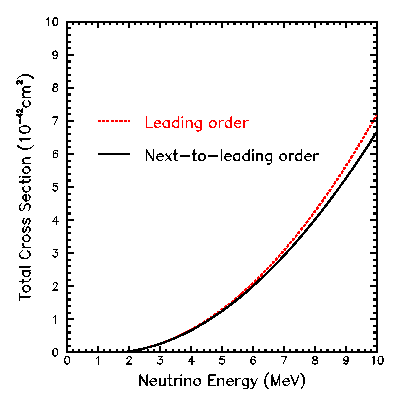
\includegraphics[width=.4\textwidth]{figures/chap1/IBD_total_cross_section.eps}
	\caption{The IBD total cross section calculated to the leading order and next-to-leading order terms.}
	\label{fig:IBD_total_cross_section}
\end{figure}

\section{Muon Induced Backgrounds}

The Earth is constantly bombarded by high energy particles known as cosmic rays. The primary source of cosmic ray is protons. When protons interact with the air molecules, secondary particles originate which in turn decay and generate muons, neutrinos, electrons and photons. Figure~\ref{figure:atmospheric_cosmic_rays} shows the vertical fluxes of the dominant cosmic ray components estimated from the intensity of primary nucleons incident on top of the atmosphere. At sea level (altitude = 0) there are still high fluxes of cosmic rays ranging from about 0.1 to 100 $m^{-2}s^{-1}sr^{-1}$. Fortunately rocks are very good natural shielding from the particles and when one goes deep enough underground only muons and neutrinos can survive. Therefore sensitive experiments go underground and the main sources of background would be the natural radioactivity from rocks as well as muons and particles or isotopes induced by muons.
\begin{figure}
	\centering
	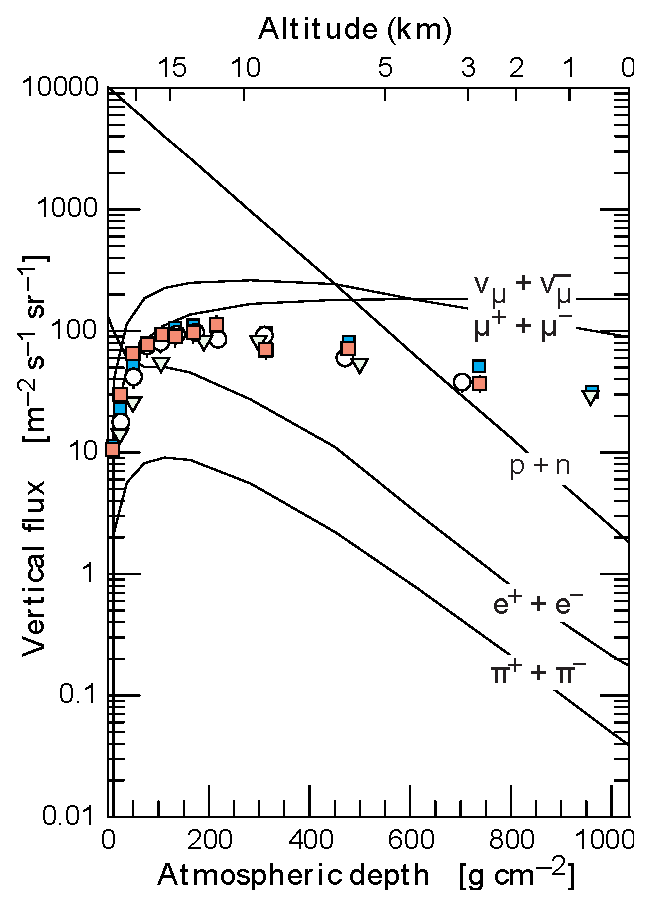
\includegraphics[width=.5\textwidth]{figures/chap1/atmospheric_cosmic_rays.eps}
	\caption{Estimated vertical fluxes of major cosmic ray components. Points are measurements of negative muons with energy larger than 1 GeV.}
	\label{figure:atmospheric_cosmic_rays}
\end{figure}

Daya Bay's experimental halls are also underground, and the muon induced neutrons and isotopes constitute one of the major background sources. For Daya Bay, the sea level muon energy and angular distribution is important because in order to get the energy and angular distribution in each hall with Monte Carlo simulation, the sea level data together with the mountain overburden profile and the rock composition is input into the simulation and the muons are then propagated through the rock to get the propagated energy and angular distribution for those survived to the ceiling of the halls. Conventionally the sea level muon flux is described by the Geisser's formula~\cite{Beringer2012},
\begin{equation}
\frac{dN_\mu}{dE_\mu d\Omega}=\frac{0.14E_\mu^{-2.7}}{cm^2\cdot s \cdot sr \cdot GeV}\left\lbrace \frac{1}{1+\frac{1.1E_\mu\cos\theta}{115GeV}}+\frac{0.054}{1+\frac{1.1E_\mu\cos\theta}{850GeV}} \right\rbrace
\end{equation}
where the two terms in the braces give the contribution of pions and kaons, respectively.
  \chapter{The Daya Bay Experiment}

\section{The Daya Bay Site}
To measure $\theta_{13}$, an experimental site with high thermal power of reactors to supply large antineutrino flux and with mountains nearby to serve as cosmic ray shielding is required. Daya Bay is the appropriate site meeting the requirements.

The Daya Bay reactor complex is located on the southeast coast of China, 55 km northeast of Hong Kong. The reactor complex is composed of 3 nuclear power plants, namely the Daya Bay (DYB) nuclear power plant, the Ling Ao (LA) nuclear power plant and the Ling Ao-II (LA II) nuclear power plant. Each nuclear power plant is equipped with a pair of functionally identical pressurized water reactors (PWR) separated by 90 m. Each reactor core supplies 2.9 GW thermal power. The Ling Ao nuclear power plant is \textasciitilde 1100 m from the Daya Bay nuclear power plant, and the Ling Ao-II is \textasciitilde 500 m from the Ling Ao. On the other hand, the Daya Bay experimental facility is composed of 3 underground experimental halls, a surface assembly building, a liquid scintillator (LS) hall and a water hall (EH4). The underground halls are connected by horizontal tunnels. The 3 experimental halls are where the antineutrino detectors and the muon detectors are installed. The experimental hall closest to the Daya Bay/Ling Ao nuclear power plant is called the Daya Bay/Ling Ao near site, or experimental hall 1/2 (EH1/EH2). The experimental hall farthest from all the reactor cores is called the Far site, or experimental hall 3 (EH3). The surface assembly building is the place where people assemble the antineutrino detector (AD), do the dry run test and other detector related work before transporting equipment underground. The LS hall is where Daya Bay's liquid scintillator and Gd-doped liquid scintillator are produced and the ADs are filled. The water hall is where the ultra purity water system is placed which supplies ultra purity water to the 3 water pools in EH1, EH2 and EH3. Figure~\ref{fig:dybsite} shows experimental facility and the 6 reactor cores. The distances from the centroids of each reactor pair to the sites is shown in Table~\ref{tab:sitecoredist}.

\begin{figure}
	\centering
	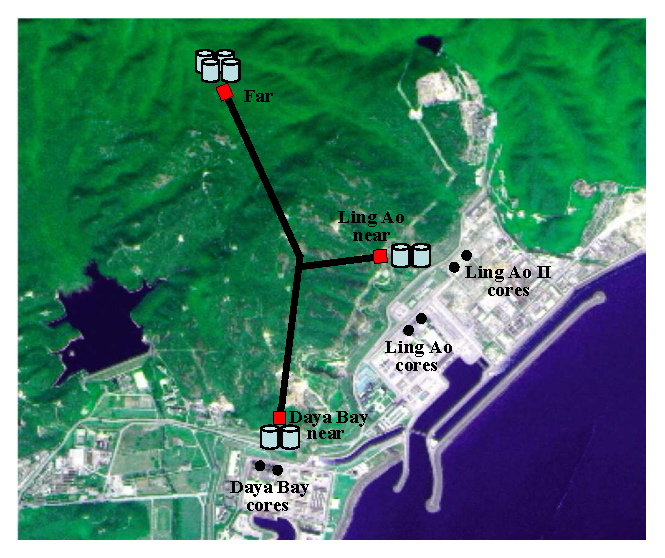
\includegraphics[width=0.45\textwidth]{figures/chap2/dayabay_site.eps}
	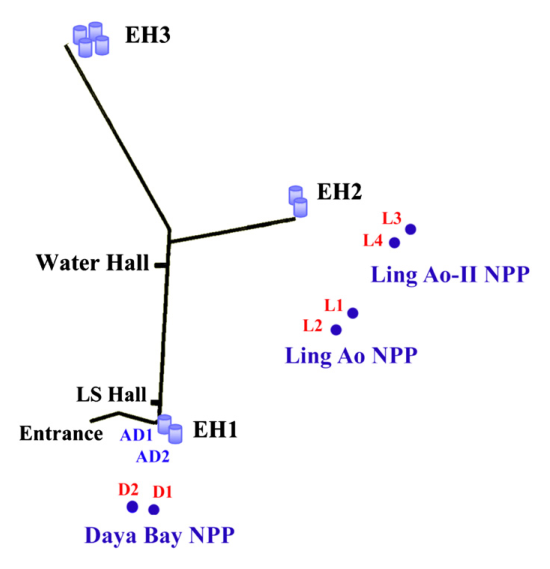
\includegraphics[width=0.35\textwidth]{figures/chap2/dayabay_site_illustration.eps}
	\caption{The Daya Bay site.}
	\label{fig:dybsite}
\end{figure}

\begin{table}
	\centering
	\begin{tabular}{|c|c|c|c|}
	\hline
	& DYB & LA & FAR \\
	\hline
	DYB cores & 363 & 1347 & 1985 \\
	\hline
	LA cores & 857 & 481 & 1618 \\
	\hline
	LA II cores & 1307 & 526 & 1613 \\
	\hline
	\end{tabular}
	\caption{Distances from the centroids of each reactor pair to the sites.}
	\label{tab:sitecoredist}
\end{table}


\section{The Antineutrino Detector}

The antineutrino detectors(ADs) are the main detectors used for detecting neutrinos via the inverse beta decay reaction. Figure~\ref{fig:CSAD} shows the cross sectional view of the design of the Daya Bay AD. The AD is separated into 3 different zones by 3 coaxial cylindrical vessels. They are the stainless steel vessel (SSV), the outer acrylic vessel (OAV) and the inner acrylic vessel (IAV) from the outside in. The SSV is a 5 m high cylinder with a 5 m diameter. The OAV is a 4 m high cylinder with a 4 m diameter while the IAV is a 3 m high cylinder with a 3 m diameter. Inside the IAV is the neutrino target filled with 20 t liquid scintillator doped with gadolinium whose concentration is $0.1\%$ by weight. 21 t of unloaded liquid scintillator (LS) is filled between the IAV and the OAV which serves as the $\gamma$ catcher. The outermost region between the IAV and the SSV is filled with 37 t of mineral oil and is call the buffer layer.
\begin{figure}
	\centering
	\includegraphics[width=0.7\textwidth]{figures/chap2/AD_cross_section.eps}
	\caption{Cross sectional view of the Daya Bay antineutrino detector.}
	\label{fig:CSAD}
\end{figure}
Each antineutrino detector is equipped with 192 8-inch Hamamatsu R5912 PMTs mounted on 8 ladders along the circumference of the SSV and within the mineral oil region.

\subsection{The Liquid Scintillator}
The liquid scintillator is 


\section{The Muon System}

To shield the ADs from backgrounds introduced by cosmic ray muons, the ADs are surrounded by muon detectors. The muon system consists of two detector subsystems. One is the water pool in which ADs are submerged which serves as a water Cerenkov counter. The other is the Resistive Plate Chamber(RPC) system which covers the water pool.

\subsection{The Water Cerenkov Detector}

When a charged particle passes through a medium at a speed faster than the speed of light in the medium, Cerenkov radiation will be generated. If PMTs are mounted inside the detector facing the medium, charged particles can be detected by the Cerenkov detector with high efficiency by counting the number of PMTs receiving Cerenkov photons.



\subsection{The Resistive Plate Chambers}

In addition to the water pool itself, the water pool is covered by another muon detector called resistive plate chamber(RPC). The RPCs are basically parallel plate gas detectors whose detailed physics will be discussed in the next chapter. This design of muon system not only increases the muon tagging efficiency but also greatly increases the accuracy of the muon track reconstruction.



\section{The Electronics, Data Acquisition and Offline Software}

For the ADs, each AD PMT raw signals are connected to the Front End Electronics boards (FEEs). Every FEE board has up to 16 channels and can do a charge integration and count for the number of PMT channels over the threshold. The system trigger can be issued by the total energy or total number of fired PMTs.

Daya Bay's offline software, NuWa, is a software framework based on Gaudi which is developed at LHCb. By definition a software framework is software which provides generic functionality and in which users can add additional user's own codes to do specific jobs.
  \chapter{The RPC Muon Detector}

The development of Resistive Plate Chamber (RPC) was first motivated by the need to improve detectors' timing characteristic. The first improvement was Pestov spark counter developed by Yu.N. Pestov and G.V. Fedotovich. Later on the great simplification of the realization of the concepts of Pestov counter introduced in 1981 by R. Santonico and R. Cardarelli~\cite{Santonico1981} leads to RPC.


\section{RPC bare chambers}
A RPC bare chamber is a parallel plate gas detector for detecting charged particles. A Daya Bay RPC bare chamber is formed by two 2 mm bakelite sheets separated by spacers to form a 2 mm gas gap. A gas combination of Ar, isobutane and R-134A flows in the gap. When charged particles pass through the gas gap, Ar molecules are ionized and the released electrons then undergo acceleration by the applied electric field. This primary electron then ionizes other Ar molecules and generates an electron avalanche. When the avalanche electrons drift the the anode, they induce electric signals which can then be readout. The isobutane can absorb ultraviolet photons and prevents a secondary streamer. The R-134A has high electron affinity and can restrict the size of the streamer.


\section{RPC Modules}
A Daya Bay RPC module is primarily composed of 4 layers of RPC bare chambers. Each layer is formed by 2 RPC bare chambers with the same length but different width. The larger RPC bare chamber has a dimension of 2.1 m $\times$ 1.1 m. The smaller one has a dimension of 2.1 m $\times$ 1.0 m. From bottom to top, the size of the RPC bare chambers alternates so as to offset the dead region due to the edge of the bare chambers. Each RPC layer is equipped with a 2.1 m $\times$ 2.1 m copper-clad FR-4 readout plane consisting of 8 readout strips. The 4 readout layers are oriented, from bottom to top, in the $x$, $y$, $y$, $x$ directions. With this readout arrangement, the position of the incident particle can be reconstructed.


\section{RPC Readout electronics}
Each strip is connected to the Front End Card (FEC).
  \chapter{Neutron Production Mechanisms in Liquid Scintillator}

Muons interact with matter through exchange of virtual photons. The generated neutrons can be categorized into two kinds, directly generated neutrons and secondary neutrons~\cite{Malgin2008}. Directly generated neutrons can be visualized with the following picture. The electromagnetic fields generated by charged particles can be thought of as a swarm of virtual photons traveling with the particles. When a muon passes by an atomic nucleus, it interacts with the nucleus by exchanging virtual photons with the nucleus. Being struck by the virtual photons, the nucleus could become excited and when it deexcites, neutrons could be released. To quantify direct neutron generation, one can first get the virtual photon frequency spectrum with Williams-Weissacker's method of virtual quanta, and then convolute with the photoneutron total cross section of the material under study.

\section{Giant Dipole Resonance}
In the photonucleus interaction cross section, the process taking place with the lowest energy is giant dipole resonance. When photons with wavelength comparable to the size of the nucleus, they see the nucleus as a whole. The oscillating electrinc field displaces the protons away from their position and a electric dipole is formed. This is a form of the excitation of the nucleus, and when the nucleus deexcites, one or more neutrons can be released.


\section{quasideutron}
With higher photon energy, the photons start to see the proton-neutron pair in the nucleus.


\section{\texorpdfstring{$\Delta$}{Delta} production}
If the photon energy goes higher, the photons can see individual nucleons and can excite the proton and form $\Delta$ resonances. Protons and neutrons can be excited to form $\Delta$ resonances with the same quark content but higher angular momentum. They decay and generate neutrons.
  \chapter{Neutron Yield}

\section{Methodology}

Ideally if one wants to measure the neutron yield by muons, one can shoot a monoenergetic muon beam at an infinite-long target and surround the target with a $4\pi$ detector which are able to identify and measure the momentum of all generated particles. This kind of idealization can be achieved closely with Daya Bay experiment.

\begin{figure}
\centering
\begin{tikzpicture}
	\draw (0,0) ellipse (.1cm and .2cm);
	\draw (0,0) ellipse (1cm and 2cm);
	\draw (0,.2) -- (3,.2);
	\draw (0,-.2) -- (3,-.2);
\end{tikzpicture}
\caption{An ideal muon induced neutron measurement} \label{fig:IdealMuN}
\end{figure}

Suppose we know the muon track with some reconstruction algorithm. For those muons passing through the inner acrylic vessel(IAV), we can form a imaginary cylinder coaxial with the track which is fully contained in the IAV. If we fix the radius of the imaginary cylinder, for each track we have to adjust its length so as to make the cylinder fully contained in the IAV. Only neutrons captured in the imaginary cylinder count. If we concatenate the imaginary cylinders one after another, the ideal experiment is approximately realized, with some differences,
\begin{enumerate}
	\item Underground muons are not monoenergetic.
	\item The imaginary cylinders serve as both the target and the detector.
	\item Generated particles are hard to detect except neutrons.
\end{enumerate}

Although most underground experiments are not designed for measuring the neutron yield by muons, a in situ measurement of neutron background is still desirable. Since the energy of the underground muons can never be controlled, instead of measuring neutron yield as a function of the incident muon energy, a common practice is to measure neutron yield as a function of the incident \emph{mean} muon energy. And since this measurement is \emph{inclusive}, we don't have to know every detail of each intermediate particle leading to neutron production.

\section{Results}
  \chapter{Conclusion}

Neutron yield by muons at Daya Bay measured with the methodology stated in the previous chapter for each experimental hall is listed in Table.


%\clearpage % start a new page for references
  %the cross section of inverse beta decay\\
The cross section of inverse beta decay is given by
\begin{eqnarray*}
\sigma& = &\frac{G_F^2E_\nu^2}{\pi}\vert\cos\theta_c\vert^2\left( 1+3\left( \frac{g_A}{g_\nu}\right)^2 \right)\\
      & = & 9.23 \times 10^{-42} \left( \frac{E_\nu}{10MeV} \right)^2 cm^2
\end{eqnarray*}

Since neutrinos come in a variety of energies, the oscillation probability
should be averaged over the whole spectrum. For a density of state $\rho(E)$,
the average oscillation probability is given by
\[
  \bar{P}_{\alpha \rightarrow \beta}(L)=\frac{1}{E_{max}}\int_0^{E_{max}}P_{\alpha \rightarrow \beta}(E)\rho(E)dE
\]
  
  \bibliographystyle{ieeetr}%Choose a bibliograhpic style
  \bibliography{mainmatter/references}
\end{document}